\chapter{Literature review}
\label{chapter8}
\setcounter{enums}{0}


\noindent This chapter surveys previous literature based on HPSG
(Head-driven Phrase Structure Grammar,
\citealt{pollard:sag:94}),\is{HPSG} MRS (Minimal Recursion Semantics,
\citealt{copestake:etal:05}),\is{MRS} and other frameworks. First,
Section \ref{8:sec:hpsg} investigates HPSG-based studies on information
structure, which are largely based on a pioneering study offered by
\citet{engdahl:vallduvi:96}.  Section \ref{8:sec:mrs} looks into how several
previous studies represent information structure using the MRS
formalism, and how they differ from the current model.
Section \ref{8:sec:phonology} surveys prior studies of how phonological
structure interacts with information structure in HPSG.
Section \ref{8:sec:other-frameworks} offers an explanation of how other
frameworks treat information structure within their formalism, and
what implications they have for the current model.


\section{Information structure in HPSG}
\label{8:sec:hpsg}


To my knowledge, \citet{engdahl:vallduvi:96} is the first endeavor to
study information structure within the HPSG framework.\is{HPSG} This
pioneering work has had a great effect on most subsequent HPSG-based
studies of information structure. The main constraints
\citet{engdahl:vallduvi:96} propose are conceptualized in
\myref{avm:engdahl:vallduvi} and \myref{avm:engdahl:vallduvi:words}.
Many HPSG-based studies on information structure, irrespective of
whether they use MRS,\is{MRS} present a variant version of
\myref{avm:engdahl:vallduvi} and \myref{avm:engdahl:vallduvi:words} as
a means of encoding information structure.  For this reason, they show
a certain degree of overlap in the way they represent information
structure and calculate information structure values.


\myexe{\enumsentence{\label{avm:engdahl:vallduvi}\evnup{
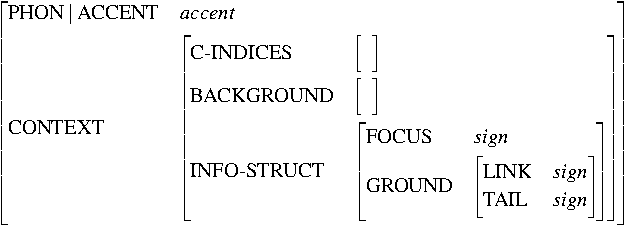
\includegraphics{pdf/engdahl-vallduvi.pdf}}}}

\myexe{\eenumsentence{\label{avm:engdahl:vallduvi:words}
\item\evnup{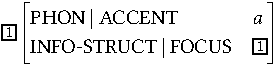
\includegraphics{pdf/engdahl-vallduvi-a.pdf}}
\item\evnup{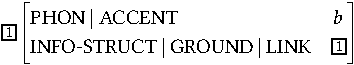
\includegraphics{pdf/engdahl-vallduvi-b.pdf}}
\item\evnup{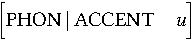
\includegraphics{pdf/engdahl-vallduvi-u.pdf}}}}


\citet{engdahl:vallduvi:96} regard information structure as an
interface across different layers in human language.  This notion can
be more precisely explained within the HPSG framework, because HPSG
accounts for various structural layers\is{HPSG} (e.g.\ phonology,
morphosyntax, semantics, and pragmatics) in an interactive
way. Regarding information structure in \ili{English},
\citeauthor{engdahl:vallduvi:96} pay particular attention to the
co-operation between phonological behaviors and contextual
information.  In their proposal, \tdl{accent} has three subtypes in
\ili{English}. They use the traditional distinction between the A and
B accents as shown in \myref{avm:engdahl:vallduvi:words}
\citep{bolinger:58,jackendoff:72}; \tdl{a} for A-accented words,
\tdl{b} for B-accented ones, and \tdl{u} for unaccented
ones.\is{A-accent}\is{B-accent} In order to determine if their
constraints work analogously cross-linguistically, they also analyze
sentences in Catalan, in which information structure is expressed
without reference to prosodic patterns. Unlike \ili{English}, Catalan
does not place a constraint on PHON to instantiate information
structure. INFO-STRUCT in Catalan, instead, is expressed via SUBCAT
(SUBCATegorization) and phrasal types of daughters.  Although their
analysis dwells on left/right \isi{dislocation} constructions in
Catalan, their approach has had a strong influence on following
HPSG-based studies, including \citet{dekuthy:00} for \ili{German},
\citet{bildhauer:07} for \ili{Spanish}, \citet{chang:02} and
\citet{chung:etal:03} for \ili{Korean}, \citet{ohtani:matsumoto:04}
and \citet{yoshimoto:etal:06} for \ili{Japanese}, and many
others.\is{HPSG}\is{left dislocation} \is{right dislocation}


These previous studies share a common proposal that information
structure is an independent module within a grammatical framework that
should be represented separately from CAT (CATegory) and CONT
(CONTent): Either under SYNSEM{$\mid$}CONTEXT
\citep{engdahl:vallduvi:96,chang:02,ohtani:matsumoto:04,yoshimoto:etal:06,paggio:09}
or outside of SYNSEM \citep{dekuthy:00,chung:etal:03,bildhauer:07}.
The current analysis, however, merges information structure into CONT
(i.e.\ MRS).\is{MRS}



On the other hand, previous studies are differentiated from each other
in the values the relevant types utilize in formalizing components of
information structure. In other words, it is necessary to determine
whether the value of the information-structure related features is a
whole sign or whether that value is something semantic
(i.e.\ MRS).\is{MRS} The traditional means of formalizing information
structure values is to use coreferences between the whole sign and a
value listed for FOC(US) and TOP(IC). \citet{engdahl:vallduvi:96} make
use of this method, and \citet{chung:etal:03} and
\citet{ohtani:matsumoto:04} utilize the same method for handling
information structure in Korean and Japanese, respectively. Recently,
several studies co-index something inside of MRS with a value in the
list of FOCUS, TOPIC, and others. In \citet{yoshimoto:etal:06},
\citet{bildhauer:07}, and \citet{sato:tam:12}, the RELS itself has a
structure-sharing with a value in the lists of components of
information structure.  \citet{paggio:09} also utilizes MRS,\is{MRS}
but the values in the lists of components of information structure are
co-indexed with the value of INDEX (e.g.\ \tdl{x1}, \tdl{e2}, etc.).
These two methods represent just two of many methods for representing
information structure in HPSG and MRS.\is{HPSG}\is{MRS} Taking a
different approach, \citet{chang:02} represents information structure
using just a string. \citet{kim:07} and \citet{kim:12a} use a boolean
feature as the value of FOCUS and TOPIC, and these features are under
an independent structure called INFO-ST.  Sometimes, a specific
feature structure is introduced, which represents logical forms
\citep{webelhuth:07,dekuthy:meurers:11}.


\subsection{Sentential forms}
\label{8:ssec:sform}


\citet{engdahl:vallduvi:96} argue that information structure is an
integral part of grammar.  In a similar vein, \citet{lambrecht:96}
regards information structure as a subtype of sentential grammar.


There exist various suggestions on how information structure affects
forms at the sentence level, such as topic-comment and
focus-\isi{ground} (i.e.\ bipartite structures).  There are two basic
components in the proposal by \citeauthor{engdahl:vallduvi:96};
\isi{focus} and \isi{ground}. While ground acts as an usher for focus,
focus is defined as the actual information or update potential of a
sentence. Ground, consisting of link and tail, is viewed as something
already subsumed by the input information state.\footnote{Note that
  ground is not the same as \isi{background}. Ground is thought of as
  opposite to focus, while background is neither focus nor
  \isi{topic}.}  This definition implies that a sentence can have a
ground if and only if the informative content guarantees its use. For
example, sentences with sentential focus (\tdl{all-focus} in 
the present study) -- such as a reply to
questions like \textit{What happened?}, are not required to include
ground.\is{background} Since they divide ground into link and tail, in
line with \citet{vallduvi:90}, they make use of a tripartite structure
consisting of different combinations of focus, link, and
tail.\footnote{\citet{buring:03} suggests another tripartite structure
  such as topic-focus-background.} Building upon some extra
constraints such as barring focus from preceding link (i.e.\ linear
order in instantiating information structure, such as link
\ensuremath{>} focus \ensuremath{>} tail), they propose four types of
sentential forms; link-focus, link-focus-tail, focus-tail, and
all-focus. For example, (\ref{exe:engdahl:vallduvi:96:5}A1) is a
link-focus construction, while (\ref{exe:engdahl:vallduvi:96:5}A2) is
a link-focus-tail construction.



\myexe{\enumsentence{\label{exe:engdahl:vallduvi:96:5}
\begin{tabular}[t]{ll}
Q1: & {So tell me about the people in the White House.} \\
    & {Anything I should know?}\\ 
A1: & {Yes. The \textbf{president} [$_{f}$ hates the
    Delft \textsc{chine set}]. Don't use it.}\\ Q2: & {In the
  Netherlands I got a big Delft china tray that matches the set}\\ & {in the
  living room. Was that a good idea?}\\ A2: & {Maybe. The
  \textbf{president} [$_{f}$ \textsc{hates}] the Delft chine set.} \\ & {(but
  the \textbf{first lady} \textsc{likes}
  it.) \citep[5]{engdahl:vallduvi:96}}\\
\end{tabular}}}


This classification is similarly implemented as a hierarchy in
\citet{paggio:09}, though the terms are different (i.e.\ \tdl{topic}
for link, and \tdl{bg} for tail). The type
hierarchy \citet[140]{paggio:09} proposes for \ili{Danish} is shown in
Figure~\ref{fig:hier:paggio}, and the lowest subtypes
are exemplified in \myref{exe:paggio} respectively.


 
\begin{figure}[!t]
\begin{center} 
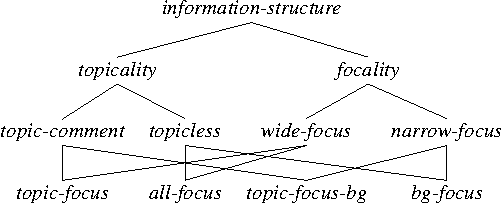
\includegraphics{pdf/paggio.pdf}
\caption{Type hierarchy of \citet{paggio:09}}
\label{fig:hier:paggio}
\end{center}
\end{figure}




\myexe{\eenumsentence{\toplabel{exe:paggio}
\item\shortex{8}
  {(Hvad & lavede & b{\o}rnene?) & [$_{T}$ & De] & [$_{F}$ & spiste & is].}
  {(what & did & children.\textsc{def}) & & they & & ate & icecream}
  {`What did the children do? They ate icecream.' (\tdl{topic-focus})}
\item\shortex{9}
  {(Hvad & spiste & b{\o}rnene?) & [$_{BG}$ & [$_{T}$ & De] & spiste] & [$_{F}$ & is].}
  {(what & ate & children.\textsc{def}) & & & they & ate & & icecream}
  {`What did the children eat? They ate icecream.' (\tdl{topic-focus-bg})}
\item\shortex{9}
  {(Hvem & har & spist & isen?) & [$_{BG}$ & Det & har] & [$_{F}$ & b{\o}rnene].}
  {(who & has & eaten & icecream.\textsc{def}) & & that & have & & children.\textsc{def}}
  {`Who has eaten the icecream? The children did.' (\tdl{bg-focus})}
\item\shortex{7}
  {(Hvad & skete & der?) & [$_{F}$ & B{\o}rnene & spiste]  & is].}
  {(what & happened & there) & & children.\textsc{def} & ate & icecream}
  {`What happened? The children ate icecream.' (\tdl{all-focus}) [dan] \citep[139]{paggio:09}}}}



The present study concurs that information structure needs to be
investigated as a subtype of sentential grammar
\citep{lambrecht:96,engdahl:vallduvi:96,paggio:09}. However, the type
hierarchy given in Figure~\ref{fig:hier:paggio} is altered in the
current analysis to accommodate a cross-linguistic perspective.  In
particular, it is necessary to delve into whether or not the hierarchy
for sentential forms has to deal with the linear order of components
of information structure.  At first glance, \tdl{bg-focus} in
Figure~\ref{fig:hier:paggio} might look inconsistent with the
focus-tail construction presented by
\citeauthor{engdahl:vallduvi:96}. As exemplified in
(\ref{exe:paggio}c), a constituent associated with \tdl{bg} can
precede other constituents associated with \tdl{focus} in
\ili{Danish}, which means the linear ordering constraint (i.e.\ link
\ensuremath{>} focus \ensuremath{>} tail) is language-specific.  The
different linear orders notwithstanding, the present study claims that
\tdl{bg-focus} in Figure~\ref{fig:hier:paggio} is actually the same as
focus-tail.  \citet{paggio:09} calls the identificational \isi{focus}
of (\ref{exe:paggio}c) \tdl{bg-focus} that serves to identify a
referent as the missing argument of an open proposition
\citep[122]{lambrecht:96}.\footnote{The \tdl{bg-focus} sentential form
  is similar to cleft constructions.\is{clefting}} For this reason,
the type hierarchy for sentential forms in the current work is built
up without an ordering constraint, exclusively considering which
components participate in forming information structure.






\subsection{Location within the feature geometry}
\label{8:ssec:hpsg:context}

Previous literature commonly introduces an independent typed feature
structure for information structure into \tdl{sign}. The independent
structure is either CXT (ConteXT) dealing with pragmatic
(i.e.\ contextual) information or just INFO-ST; \citet{chang:02}
employs PRA{$\mid$}DF{$\mid$}TFA in \myref{avm:chang:pra},
\citet{ohtani:matsumoto:04} uses CONX{$\mid$}INFO-ST, and
\citet{kim:07} uses just INFO-ST immediately under \tdl{sign}. Similar
structures are used in other papers:
SYNSEM{$\mid$}LOC{$\mid$}CONTEXT{$\mid$}INF-ST
\citep{yoshimoto:etal:06}, SYNSEM{$\mid$}IS \citep{bildhauer:cook:10},
CTXT{$\mid$}IS \citep{bjerre:11}, INFO-STRUC
\citep{dekuthy:meurers:11}, etc.  The functionality of these features
has one thing in common: Information structure is separately
represented from both morphosyntactic structure (i.e.\ CAT) and
semantic structure (i.e.\ CONT).




Information structure as presented here is an independent module in
grammar, however, that does not necessarily mean that information
structure should be separately represented on AVMs. Unless there is a
necessity to separate components of information structure from
CONT(ent), the independent structure is redundant.  In seeking a
minimal solution, is it possible to represent information structure
without introducing additional structure?  \citet{partee:91} also
addresses this with her observations that information structure is not
independent of truth-conditions.\is{truth-conditions} If information
structure is truth-conditionally relevant, it should be represented in
the semantics.  \citet{engdahl:vallduvi:96}, nevertheless, invoke
a separate representation in the belief that information structure and
logical semantics have to be represented in the grammar in a modular
manner. They leave the final resolution of these two components as a
question for future work.\is{HPSG} My understanding is that most
subsequent HPSG-based studies on information structure do not attempt
to answer how final meanings are arrived at.\footnote{To my knowledge,
  one exceptional study is \citet{webelhuth:07}, in which information
  structure components are dealt with under CONT.}  The next chapter
shows information structure can be fully represented without using
CTXT or introducing an independent structure.




Representing information structure within CONT (i.e.\ MRS)\is{MRS} has
another important merit in the context of multilingual machine
translation. As stated earlier, the present study argues that
translation means reshaping the packaging of the information of a
sentence.  Thus, one of the most important considerations in
representing information structure is its availability in multilingual
machine translation as a computational model. Because all ingredients
relevant to translation must be accessible in MRS within our
\isi{transfer-based} system \citep{oepen:etal:07}, information
structure should be accessible in MRS.




\subsection{Underspecification}
\label{8:ssec:underspecification}


One of the main motivations for and advantages in using the HPSG/MRS
formalism is \isi{underspecification}.  The value of a particular
attribute can be left underspecified in a description unless a
constraint identifies the value with a more specific type.  This makes
grammatical operation more flexible and more economical. For example,
(\ref{avm:engdahl:vallduvi:words}c) means that unaccented words leave
their information structure value underspecified, facilitating varied
meanings of an unmarked expression.\is{HPSG} \citet{kuhn:96} argues
that using \isi{underspecification} is a more effective way to
represent information structure; especially for the purpose of
implementing HPSG-based NLP applications (e.g.\ machine translation,
\isi{TTS} (Text-To-Speech) systems, etc.).  However,
underspecification has been scarcely used in previous HPSG-based
studies on information structure.  The current model relies on
underspecified values of components of information structure.  More
specific justifications as to why underspecification is crucial for
representing information structure are discussed in the following
subsections.


\subsubsection{Prosody}
\label{8:ssec:hpsg:prosody}

In most HPSG-based studies of information structure, a typed feature
structure for representing prosody is commonly introduced.\is{prosody}
The interface between information structure and prosody has been
studied for many Indo-European languages as well as in
non-Indo-European languages such as Korean and Japanese.
\myref{avm:chang:prosody}, taken from \citet{chang:02}, stands for a
typed feature structure for prosody in Korean which has two key
attributes TC (Terminal Contour) and STR (STRess). The values of the
former include falling (HL\%), neutral (H\%), and rising (LH\%), and
those of the latter stand for four levels of stress.



\myexe{\enumsentence{\label{avm:chang:prosody}\evnup{
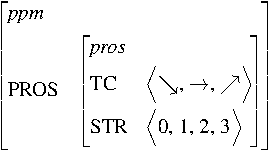
\includegraphics{pdf/chang-prosody.pdf}}}}

\noindent In his formalism, this structure has a correlation with
another typed feature structure, namely PRA (PRAgmatics). Information
structure values, such as topics and foci, are gathered into the lists
under PRA{$\mid$}DF{$\mid$}TFA as presented in
\myref{avm:chang:pra}\footnote{DF stands for Discourse Function, and
  TFA means Topic-Focus Articulation. Additionally, SA is short for
  Speech Act, BKG is for BacKGround, POV is for Point-Of-View, and CTR
  is for CenTeR.\is{background}}.

\myexe{\enumsentence{\label{avm:chang:pra}\evnup{
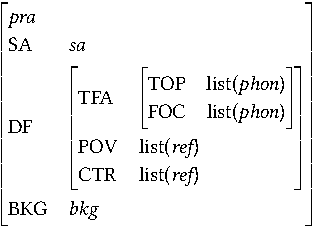
\includegraphics{pdf/chang-pra.pdf}}}}

\newpage 
\noindent For example, \nun and \ika in Korean have one of the feature
structures presented in (\ref{avm:chang:tf}a) and
(\ref{avm:chang:tf}b), respectively.  In \myref{avm:chang:tf}, the
PHON structure is the same as the STEM structure in
\texttt{matrix.tdl} of the \lingo \isi{Grammar Matrix} system. That is, the
value type of PHON is just string. Despite the name, it is not
directly related to any 
phonological information.\is{contrastive topic}\is{contrastive focus}\is{narrow focus}


\myexe{\enumsentence{\toplabel{avm:chang:tf} 
\begin{tabular}[t]{lllllll}
a. & i. & Zero Topic & & b. & i. & (Narrow) Focus \\ & &
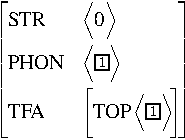
\includegraphics{pdf/chang-zt.pdf} & & & &
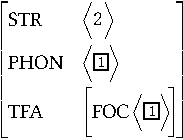
\includegraphics{pdf/chang-nf.pdf} \\ & ii. & (Thematic) Topic & & &
ii. & Contrastive Focus \\ & & 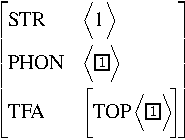
\includegraphics{pdf/chang-tt.pdf} & &
& & 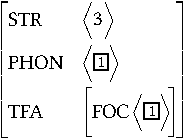
\includegraphics{pdf/chang-cf.pdf} \\ & iii. & Contrastive Topic
\\ & & 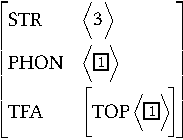
\includegraphics{pdf/chang-ct.pdf} \\
\end{tabular}}}




\noindent \citet{ohtani:matsumoto:04}, similarly, analyzed \wa-marked
and \ga-marked NPs in Japanese: \textit{Wa}-marked NPs are interpreted
as either \isi{topic}, restrictive \isi{focus} or non-restrictive
focus,\footnote{In \citet[95]{ohtani:matsumoto:04}, restrictive
  focus means wide focus.\is{wide focus}}  whereas \ga-marked NPs are interpreted as
either restrictive focus or all focus.  Similarly to
\myref{avm:chang:tf} in Korean, in the formalism
\citeauthor{ohtani:matsumoto:04} propose \wa and \ga can have one of
the feature structures in (\ref{avm:ohtani:matsumoto:wa:ga}a) and
(\ref{avm:ohtani:matsumoto:wa:ga}b), respectively.

\myexe{\enumsentence{\toplabel{avm:ohtani:matsumoto:wa:ga} 
\begin{tabular}[t]{lll}
a. & i. & \evnup{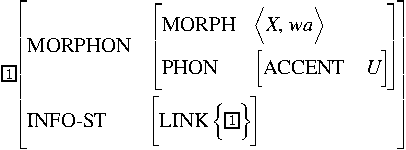
\includegraphics{pdf/ohtani-matsumoto-wa1.pdf}} \\
   & ii. & \evnup{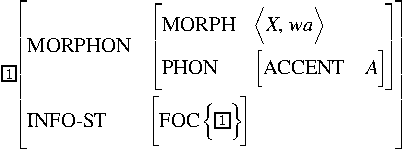
\includegraphics{pdf/ohtani-matsumoto-wa2.pdf}} \\
\end{tabular}
\newline
\begin{tabular}[t]{lllllll}
b. & i. & \evnup{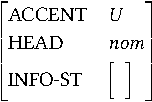
\includegraphics{pdf/ohtani-matsumoto-ga1.pdf}} &
ii. & \evnup{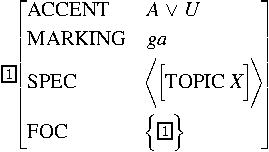
\includegraphics{pdf/ohtani-matsumoto-ga2.pdf}} \\
 & iii. &
\evnup{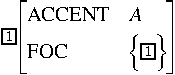
\includegraphics{pdf/ohtani-matsumoto-ga3.pdf}}
\end{tabular}}}



\myref{avm:chang:tf} and \myref{avm:ohtani:matsumoto:wa:ga}, though
their formats are slightly different, are actually the Korean and
Japanese variants of \myref{avm:engdahl:vallduvi:words} in
\ili{English}.  \citet{bildhauer:07} argues that it is rather unclear
where the information about accents comes from.  This criticism seems
appropriate when we think of the current computational environments
for sentence processing. Because our applications are mostly
text-based, for now it would be quite difficult to resolve for accent
type within the text domain. Nonetheless, the criticism seems rather
shortsighted when we consider the future direction of language
applications.\is{HPSG} Even in the absence of an implementation that
connects the HPSG grammar to ASR (Automatic Speech Recognition)
systems to prosody extraction or \isi{TTS} (Text-To-Speech) systems
with prosody generation,\is{prosody} if there is a robust correlation
between information structure and prosodic accents, the grammar can
leverage information about stress to yield higher performance. Hence,
it is important to allow the grammar formalism to model prosodic
information using \isi{underspecification} \citep{kuhn:96}. I believe
that this strategy contributes to the long-term task of refining
meaning representation via prosodic information.



However, there is a remaining controversial point embedded in
\myref{avm:chang:tf} and \myref{avm:ohtani:matsumoto:wa:ga}.  In fact,
they are tantamount to redundantly introducing \ika and \nun in
Korean, and \ga and \wa in Japanese into the lexicon. For example,
(\ref{avm:chang:tf}a) implies that the morphemes for introducing a
zero \isi{topic} \nun, a thematic topic \nun, and a \isi{contrastive
  topic} \nun are three separate homonyms.  The use of multiple rules
for \nun and \wa is an undesirable choice which should be avoided if
possible.  Korean and Japanese very productively employ \nun and \wa,
respectively, which means that having multiple lexical entries for \wa
and \nun items in the respective grammars causes problematic amounts
of spurious ambiguity.\footnote{Exploring the \textit{Sejong} Korean
  Treebank reveals that subjects in Korean are combined with \nun more
  than twice than the ordinary nominative marker \ika.} In other
words, if we include all the rules in (\ref{avm:chang:tf}a), every
\onun-marked constituent produces spurious parse trees.  As a result,
the number of parse trees can sometimes grow too large to
handle.\footnote{In fact, this is one of the major problems that cause
  a bottleneck in parsing and generation in the old version of Korean
  Resource Grammar.  It had two types of \nun; one for topic, and the
  other for contrast.\is{contrast} These two \nun sometimes had an
  adverse effect on system performance.  Occasionally, even not a long
  sentence could have a large number of parse trees if \nun occurs
  multiple times in the sentence. Accordingly, the sentence could not
  be generated in most cases because of memory overflow. For more
  information, see \citet{song:etal:10}.}  If there is something that
the multiple-entry approach captures that the single-entry approach
does not, then we should use the former, because there could be a loss
in information processing. Yet, as discussed hitherto, the lexical
markers (e.g.\ \nun and \wa) and the prosodic patterns each contribute
only partial information. In other words, neither of them can be a
decisive clue for identifying which information structure meaning is
assigned to a given constituent.



To sum up, my alternate approach for constraining lexical markers
(especially in Japanese and Korean) is as follows:\is{lexical markers}
First, there is one and only one entry for each marker. Second, the
lexical rules include prosodic structures in principle, but they are
preferentially underspecified. Third, the meaning that each marker
potentially conveys is flexibly and tractably represented to cover all
the partial information.



\subsubsection{Ambiguity}
\label{8:ssec:hpsg:boolean}


In many previous studies across theories of grammar, so-called
F(ocus)-marking is represented as a boolean feature (i.e.\ [FOCUS
  \tdl{bool}]) as proposed in \citet{zubizarreta:98}.  Handling
information structure via a boolean feature is also common in other
unification-based frameworks. For instance, \citet{choi:99}, within
the framework of \isi{LFG} (Lexical-Functional Grammar
\citealt{bresnan:01}), makes use of [\ensuremath{\pm} New] and
[\ensuremath{\pm} Prom] as presented later in \myref{fig:choi}.  Other
components of information structure are also similarly marked.  These
include [TOPIC \tdl{bool}], [CONTRAST \tdl{bool}], [HIGHLIGHT
  \tdl{bool}], and so on. For instance, \citet{kim:07} claims that
\textit{beer} in (\ref{exe:kim:beer}A) is constrained as in
\myref{avm:kim:beer}. Since \textit{beer} in (\ref{exe:kim:beer}A)
is contrastively focused (i.e.\ an answer to an alternative question
\citealt{gryllia:09}),\is{contrastive focus} it has both [HIGHLIGHT +]
and [FOCUS +] in his analysis. Note that [HIGHLIGHT \tdl{bool}] in
\myref{avm:kim:beer} indicates whether or not the constituent conveys
a contrastive meaning, which is almost the same as [CONTRAST
  \tdl{bool}].


\myexe{\enumsentence{\label{exe:kim:beer}
\begin{tabular}[t]{ll}
Q: & {Did John drink beer or coke?}\\ 
A: & {John drank beer. \citep[229]{kim:07}}\\
\end{tabular}}}

\myexe{\enumsentence{\label{avm:kim:beer}\evnup{
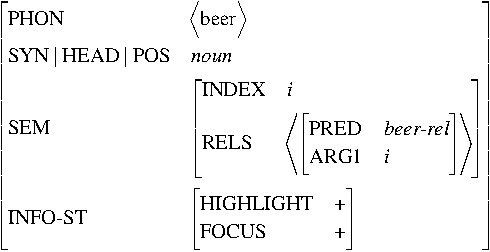
\includegraphics{pdf/kim-beer.pdf}}}}


In contrast, the present work does not use boolean features for
representing information structure meaning. This is mainly because
using boolean features would not allow us to represent information
structure as a relationship between an entity and a clause. The
current work encodes information structure into the semantic
representation via \isi{ICONS} (Individual CONStraints).\is{Individual CONStraints}
The main motivation for \isi{ICONS} is the ability to
encode information structure values as a relationship with the clause
an information structure-marked constituent belongs to, rather than as
simply a property of the constituent itself.  Chapter~\ref{chapter9}
provides the fundamentals of \isi{ICONS} in detail.




\subsection{Marking \vs meaning}
\label{8:ssec:hpsg:makring-meaning}

Most of the previous formalisms are exclusively concerned with
markings, as the name F(ocus)-marking implies.  Hence, they are rather
ill-suited to deal with any discrepancies between the forms expressing
information structure and the meanings expressed.\is{lexical markers}
The lexical markers \wa and \nun in Japanese and Korean are typical
cases showing this kind of mismatch, and \myref{avm:kim:beer}
illustrates via an example from Korean.  If \nun in Korean is used
contrastively and an NP with it is focused,\is{contrast} then the NP in
\citeauthor{kim:07}'s AVMs would be constrained as either (i) [HIGHLIGHT +,
  TOPIC +] focusing on the NP-marking system or (ii) [HIGHLIGHT +,
  FOCUS +] putting more weight on the meaning. Another potential
constraint on the NP would be [HIGHLIGHT +, FOCUS +, TOPIC +], but
this analysis fails with respect to the basic assumption the present
study is built on: topic and focus are mutually exclusive.\footnote{As
  stated earlier, there exist counterarguments to this generalization
  \citep{krifka:08}.}



The present study proposes two strategies as an alternative method.
First, information structure markings should be separately specified
from information structure meanings. The former should be constrained
using a morphosyntactic feature that can be language-specific. The
latter should be attributed within the semantics (i.e.\ under CONT),
and rely on a cross-linguistically valid type hierarchy. Second, there
are more than a few cases in which we cannot convincingly say which
element is associated with which information structure meaning.
Therefore, it is necessary to specify information structure values as
flexibly as possible. This is particularly important when creating a
robust computational model of information structure.




\section{Information structure in MRS}
\label{8:sec:mrs}


The present study, unlike previous HPSG-based studies including
\citet{engdahl:vallduvi:96}, does not introduce another structure and
instead represents information structure within the MRS semantic
representations.\is{MRS} There are two motivations for doing so. The
first motivation is that information structure impacts semantic
properties. As discussed previously, information structure
(especially, semantic \isi{focus}) is sometimes relevant to
\isi{truth-conditions} \citep{gundel:99} and scopal interpretation
\citep{buring:97,portner:yabushita:98,erteschik:99,erteschik:07,bianchi:frascarelli:10}.
Hence, it is right to incorporate information structure into the
meaning representation in a direct manner.  The second motivation is
strictly practical: The \isi{infrastructure} for machine translation
does MRS-based transfer \citep{oepen:etal:07}, therefore encoding
information structure into MRS facilitates its immediate availability
for use in machine translation.\is{transfer-based}



\largerpage[-1]
Previous HPSG-based studies can be divided into two subgroups: One
represents information structure without reference to MRS
\citep{dekuthy:00,chang:02,chung:etal:03,ohtani:matsumoto:04,webelhuth:07,kim:07,kim:12a},
and the other links information structure values in an independent
typed feature structure to MRS (e.g.\ INDEX or RELS)
\citep{wilcock:05,yoshimoto:etal:06,paggio:09,bildhauer:cook:10,sato:tam:12}.



\citet{wilcock:05}, to my knowledge, is the first attempt to use MRS
for representing information structure, modeling the scope of
\isi{focus} analogously to \isi{quantifier} scope
(i.e.\ HCONS).\is{MRS}


\myexe{\eenumsentence{\label{exe:wilcock}
\item{The president [$_{f}$ hates the china set].}
\item{1:the(x,2), 2:president(x), 3:the(y,4), 4:china(y), 4:set(y),
  5:hate(e,x,y)\\ TOP-HANDLE:5, LINK:{1}, FOCUS:{3,5} (wide focus)}}}



\noindent This is similar to the basic idea of the current analysis,
in that information structure can be represented as a list of binary
relations in the same way as HCONS is.\is{binary relation} The
difference between \citeauthor{wilcock:05}'s proposal and that of the
current analysis is that information structure in his model is
represented as handles, whereas the current model represents the
relationships between individuals and clauses as binary
relations. This facilitates scaling to multiclausal constructions. For
instance, (\ref{exe:wilcock}b) taken from \citet[275]{wilcock:05}
represents the wide \isi{focus} reading of (\ref{exe:wilcock}a)
(i.e.\ from 3 to 5). Note that in this representation, LINK
(\tdl{topic} in this paper) and FOCUS have no relation to the clause
or its head (\textit{hate}).\is{topic}





\citet{yoshimoto:etal:06} use MRS,\is{MRS} too. In their model,
information structure values are unified with whole MRS predications
rather than just indices. Based on this assumption, they apply the
information structure values to analyzing floating quantifiers in
Japanese.  However, their AVM does not look like a standard MRS
representation, and it is rather unclear how their model could be used
for practical purposes.



\citet{paggio:09} also models information structure with reference to
the MRS formalism, but the components of information structure in
\citeauthor{paggio:09}'s proposal are represented as a part of the
context, not the semantics. Though each component under
CTXT\ensuremath{\mid}INFOSTR involves co-indexation with individuals
in MRS, her approach cannot be directly applied to the \isi{\logon} MT
\isi{infrastructure} which requires all transfer-related ingredients
to be accessible in MRS \citep{oepen:etal:07}.


\largerpage[-2]
\citet{bildhauer:cook:10} offer another type of MRS-based
architecture:\is{MRS} Information structure in their proposal is
represented directly under SYNSEM (i.e.\ SYNSEM\ensuremath{\mid}IS)
and each component (e.g.\ TOPIC, FOCUS) has a list of indices
identified with ones that appear in EPs in RELS, which is not
applicable to the \isi{\logon} \isi{infrastructure} for the same
reason as the \citet{paggio:09} model.\footnote{This, of course, does
  not mean that every grammar should be compatible with the
  \isi{\logon} infrastructure. The ultimate goal of the present study
  is creating a computational library within the Grammar Matrix, which
  can be effectively used to enhance performance of HPSG/MRS-based MT
  systems. Given that \isi{\logon}, for now, is the readily available
  infrastructure for the purpose, the present study follows the
  requirements as far as possible.}



Among the various methods presented so far, the method used by the
present study most closely resembles that of \citet{paggio:09} in that
individuals (the value type of INDEX) are constrained for
representation of information structure (i.e.\ Individual
CONStraints).\is{Individual CONStraints} The main differences between
\citeauthor{paggio:09}'s approach and mine are as follows: First, I
place the feature whose value represents information structure inside
of CONT. Second, I represent information structure values using a type
hierarchy of \tdl{info-str}.\is{\textit{info-str}} Third, the features
to represent information structure involve a \isi{binary relation}
between individuals and clauses. Chapter~\ref{chapter10} enters into
the implementation details.




\section{Phonological information in HPSG}
\label{8:sec:phonology}

Quite a few HPSG-based studies explore the effect of phonological
behaviors on the structuring of information in a sentence.  However,
this subsection surveys only \citeauthor{bildhauer:07}'s
proposal.\is{HPSG}


Though the current model does not devote much attention to
phonological constraints on information structure, it is still
necessary to formalize some prosodic information in relation to
information structure markings for at least two reasons. First,
\isi{focus projection} has been considered to be triggered by
prosody. Second, as \citet{kuhn:96} and \citet{traat:bos:04} point
out, \isi{TTS} (Text-To-Speech) synthesizers and automatic speech
recognizers can be improved by using information structure. Thus, it
is my expectation that including prosodic information in the HPSG
formalism facilitates the use of HPSG-based grammars for those kinds
of systems in the long term.


\largerpage[2]
According to the account of \citet{bildhauer:07}, there are three
HPSG-based approaches to phonology; (i) metrical tree-based approaches
\citep{klein:00,haji:03}, (ii) grid-only approaches
\citep{bonami:delais:06}, and (iii) hybrid approaches that take
advantage of the two former approaches (\citeauthor{bildhauer:07}'s
own).  According to \citet[160]{bildhauer:07}, the metrical tree-based
approach provides a representation of prosodic consistency, but
deploys only nested structure. This is a drawback when it comes to
handling intonational tunes.  \citeauthor{bildhauer:07} also argues
that while the grid-only approach of \citeauthor{bonami:delais:06}
involves a basically flat representation, it is too language-spe\-cif\-ic
to be straightforwardly applied to other languages. The three basic
approaches outlined by \citeauthor{bildhauer:07} each yield their own
explanation about how phonological information can be calculated
within the HPSG framework in a general sense, and how the information
co-operates with information structure.

\largerpage[2]
Another approach to the HPSG-based interface between prosody and
syntax is provided in \citet{yoshimoto:00}.\is{prosody} Its basic
assumption is that P(rosodic)-structure and C(onstituent)-structure
form a bistratal phase with each other. The bistratal approach is not
considered in the present study for two reasons. First,
\citeauthor{yoshimoto:00}'s proposal is not directly concerned with
information structure. Second, although the interaction between
prosodic and syntactic structures is examined, the analysis is rather
language-specific (i.e.\ for Japanese) as implied by the name of the
typed feature that plays the key role (MORA).



The present analysis, largely accepting the hybrid approach, keeps an
eye towards being compatible with the HPSG-based formalism
\citet{bildhauer:07} proposes.  \citeauthor{bildhauer:07}'s account is
divided into two layers. One is the PHON list which is an immediate
feature of \tdl{sign}, made up of four components; (i) prosodic word,
(ii) phonological phrase, (iii) intonational phrase, and (iv)
phonological utterance. The other layer is intonation, which takes
charge of (v) pitch accents,\is{focus prominence} and (vi) boundary
tones. Building upon their operation, a schema of \isi{focus} prominence
rules is suggested, mainly concentrating on the top level of prosodic
hierarchy (i.e.\ phonological utterance). \citeauthor{bildhauer:07}'s
formalism develops from \citeauthor{klein:00}'s proposal that the
level of syllables does not matter, and instead the prosodic hierarchy
is represented by prosodic words (\tdl{pwrd}) and leaners
(\tdl{lnr}). The elementary unit of PHON is \tdl{pwrd}, whose skeleton
is sketched out in \myref{fig:bildhauer:pwrd-or-lnr}
\citep[161]{bildhauer:07}.\footnote{In
  \myref{fig:bildhauer:pwrd-or-lnr}, the value of SEGS is a list of
  segments.}

\myexe{\enumsentence{\label{fig:bildhauer:pwrd-or-lnr}\evnup{
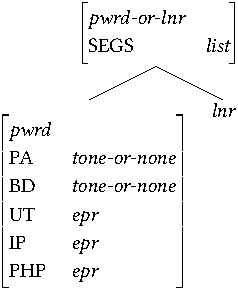
\includegraphics{pdf/pwrd-or-lnr.pdf}}}}

  
First, the lowest three features within \tdl{pwrd} in
\myref{fig:bildhauer:pwrd-or-lnr} represent prosodic hierarchical
levels above prosodic word; PHP stands for PHonological Phrase, IP is
for Intonational Phrase, and UT is the abbreviation for phonological
UTterance. Each of them has \tdl{epr} meaning Edges and Prominence as
its value type, whose typed feature structure is provided in
\myref{fig:bildhauer:epr}; LE stands for Left Edge, RE for Right Edge,
and most importantly DTE for Designated Terminal Element. Grounded
upon the prosodic rules that \citet[181]{bildhauer:07} creates, PHP, IP,
and UT are defined by a relational constraint, which places a
restriction on LE, RE, and DTE values of \tdl{pwrd} objects and
thereby specifies the relation that a prosodic word has to higher
prosodic constituents.



\myexe{\enumsentence{\label{fig:bildhauer:epr}\evnup{
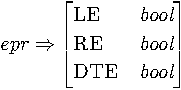
\includegraphics{pdf/epr.pdf}}}}


Second, pitch accents (PA) and boundary tones (BD), which carry
intonational information, take \tdl{tone-or-none} as their value
type. \citet[183--184]{bildhauer:07} provides the hierarchy of
\tdl{tone-or-none} in \ili{Spanish} as follows, which is to be further
revised for better cross-linguistic coverage in the present study.
Each type name on the bottom line is an element in the ToBI
format. For example, \tdl{high} means H, \tdl{low} means L, and
\tdl{low-high-star} means L+H* (i.e.\ the B-accent in \ili{English},
\citealt{bolinger:61,jackendoff:72}).\is{B-accent}


\myexe{\enumsentence{\label{fig:bildhauer:tone-or-none}\evnup{
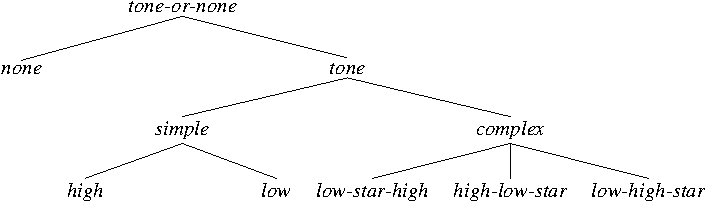
\includegraphics[width=.9\textwidth]{pdf/tone-or-none-spa.pdf}}}}


\noindent Those pitch accents and boundary tones are related to
\tdl{pwrd}, whose relationship is ruled as follows.  Pitch accents are
attached to phonological phrases, and boundary tones are connected to
intonational phrases \citep{steedman:00}.


\newpage 
\myexe{\eenumsentence{\label{avm:bildhauer:rules}
\item\evnup{{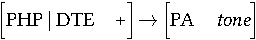
\includegraphics{pdf/php-plus.pdf}}}
\item\evnup{{
\includegraphics{pdf/php-minus.pdf}}}
\item\evnup{{
\includegraphics{pdf/ip-plus.pdf}}}
\item\evnup{{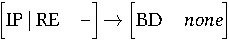
\includegraphics{pdf/ip-minus.pdf}}}}}



Given that \citet{bildhauer:07} provides a cross-linguistically
convincing proposal as such, the type hierarchy of \tdl{tone} and the
typed feature structure for phonological structure are described in
\texttt{matrix.tdl}.  Although the current work is not deeply
concerned with prosodic realizations of information structure,
information relevant to those realizations should be included into the
system as it's a common structure in human languages. This is highly
motivated by the necessity to refer to prosodic patterns for further
refinement of meaning representation in future studies.



However, the specific phonological rules given in
\myref{avm:bildhauer:rules} are only selectively implemented in the
current work. For instance, in the following chapters, two
hypothetical suffixes are used for indicating the A and B accents in
\ili{English} for ease of processing.  The rules for them are in
accordance with what \citet{bildhauer:07} proposes. However, no other
rules use that phonological information. There are two reasons for
this.\is{prosody} First, for many languages, the correlation between
prosody and information structure is not fully tested and thereby
remains unclear. Thus, I leave it to future users of the current model
to create these (potentially language-specific) rules. Second, since
the current model does not make use of any acoustic system, it is
almost impossible for the current model to implement and test
\citeauthor{bildhauer:07}'s phonological rules in a comprehensive way.

 \largerpage[-1]
\section{Information structure in other frameworks}
\label{8:sec:other-frameworks}


\subsection{CCG-based studies}
\label{8:ssec:ccg}

The \isi{CCG} (Combinatory Categorial Grammar, \citealt{steedman:01})
framework, which provides a detailed analysis of the relationship
between intonation and other structures (e.g.\ syntax, semantics, and
pragmatics), has addressed information structure since the early days
of the theory \citep{steedman:00}.\footnote{CCG departing from CC
  (Categorial Grammar) has two versions of formalism, whose history of
  progress is also deeply related to incorporating information
  structure into the formalism. The first development of CG theories
  is called UCG (Unification Categorial Grammar, \citealt{zeevat:87}),
  which employs an HPSG-style typed feature structures
  (i.e.\ \tdl{sign}). The HPSG-style formalism facilitates more
  efficient co-operation of interface across grammatical layers
  (e.g.\ syntax, semantics, etc.). The second development is UCCG
  (Unificational Combinatory Categorial Grammar,
  \citealt{traat:bos:04}), which integrates CCG and UCG, and then adds
  DRT (Discourse Representation Theory, \citealt{kamp:reyle:93}) into
  the formalism, in order to facilitate a compositional analysis of
  information structure.  Roughly speaking, those categorial grammars
  replace phrasal structure rules by lexical categories and general
  combinatory rules. In other words, the CCG framework associates
  syntactically potent elements with a syntactic category that
  identifies them as functors. There are two major rules to combine
  functional categories and their arguments, which specify
  directionality such as (i) forward application represented as
  `\ensuremath{>}' and (ii) backward application represented as
  `\ensuremath{<}'.} Consequently, one of the main characteristics of
CCG is that it is particularly and deeply oriented toward information
structure. Moreover, several CCG-based studies have accounted for how
categories of information structure in CCG can be of use for practical
systems from the standpoint of computational linguistics.


The components of information structure that \citet{steedman:00} and
\citet{traat:bos:04} introduce include theme (i.e.\ \isi{topic}), and rheme,
and \isi{focus}. There are three structures that coincide with each other:
(a) surface structure, (b) information structure, and (c) intonation.
Among these, only (c) has significance for combinatory prosody,
consisting of (c-1) pitch accents and (c-2) boundary tones. Whereas
pitch accents are viewed as properties of words, boundary tones are
defined as a boundary between theme and rheme categories.  A sequence
of one or more pitch accents followed by a boundary is referred to as
an intonational phrasal tune.


\largerpage
Pitch accents and boundary tones in CCG are mostly represented in the
ToBI format as follows.  There are six pitch accents to mark theme and
rheme, for example L+H*, L*+H for theme and H*, L*, H*+L, and H+L* for
rheme. Boundary tones are what make a clear difference between
\citeauthor{steedman:00}'s analysis and others in that he considers
them to be crucial to specifying phrasal type and thereby configuring
information structure.  Intermediate phrases consist of one or more
pitch accents, followed by either the L or the H boundary, also known
as the phrasal tone. Intonational phrase, on the other hand, consists
of one or more intermediate phrases followed by an L\% of H\% boundary
tone. Therefore, in \citeauthor{steedman:00}'s analysis of information
structure in \ili{English}, the L+H* and LH\% tune is associated with
the theme, and the H* L and H* LL\% tunes are associated with the
rheme. For instance, a surface structure \textit{Anna married Manny.}
can be analyzed as follows \citep[302]{traat:bos:04}.



\myexe{\eenumsentence{\toplabel{exe:traat:bos:04}
\item \textbf{Anna} [$_{f}$ married [$_{f}$ \textsc{Manny}]].
\item Anna L+H* LH\% married Manny H* LL\%}}


\noindent In (\ref{exe:traat:bos:04}a), \textbf{Anna} bears the
B-accent (i.e.\ L+H*), \textsc{Manny} bears the A-accent (i.e.\ H*),
and the \isi{focus} can be projected into either the NP \textsc{Manny}
itself or the VP \textit{married
  \textbf{Manny}}.\is{A-accent}\is{B-accent} In
(\ref{exe:traat:bos:04}b), the \isi{topic} meaning that
\textit{\textsc{Anna}} conveys comes from a pitch accent (L+H* after
the word), and the focus meaning that \textit{\textbf{Manny}} delivers
comes from another pitch accent (H*). A boundary tone (LH\%) forms a
border of theme. Finally, \textit{married} without any boundary tone
(i.e.\ an invisible boundary as an edge of an unmarked theme) is
included in the rheme, but it creates an ambiguous meaning with
respect to the \isi{focus} domain. \citet{traat:bos:04} represent
(\ref{exe:traat:bos:04}b) into the CCG-based formalism, in which three
information structure values \ensuremath{\theta}, \ensuremath{\rho},
and \ensuremath{\phi} are used for theme, rheme, and phrase,
respectively. Those values are used as the value types of INF
(INFormation structure), and focus is independently represented as a
boolean type.



The CCG-based studies have several key implications for my
work. First, they pay particular attention to the creation of a
computational model for information structure with an eye toward
implementing applications from the beginning.  In particular,
\citet{traat:bos:04} argue that an information structure-based
computational model should be used for both parsing and generation,
and conduct an experiment to verify that their model works.  The
information structure-based model used here was created with the same
considerations in mind. This computational model, developed in the
context of \isi{grammar engineering}, can be used not only for parsing
human sentences into semantic representations but also for generating
sentences using that representation.  Second,
\citeauthor{traat:bos:04} make use of prosodically annotated strings
as input for their experiment, because current automatic speech
recognizers do not provide enriched prosodic information.  In the
current experiment, I employ two suffixes (e.g.\ 	\textit{-a} for the
A-accent, 	\textit{-b} for the B-accent) that hypothetically represent
prosodic information (see Section \ref{12:sec:machinery}).  Though I am not
working with naturally occurring speech, the 	\textit{-a} and 	\textit{-b} suffixes
are inspired by prosodic annotation.  Lastly, the CCG-based studies
include prosodic information in their formalism in a fine-grained way
and also create linguistic rules in which prosodic information and
information structure interact with each other in a systemic way.  My
model does not yet fully use prosodic information for the reasons
discussed in Section \ref{8:sec:phonology},\is{prosody} but future work will
look at how to systematize the interaction between prosody and
information structure, taking CCG-based work as a starting point and
guide.  Although the current model is mainly concerned with text
processing, it could work through acoustic analysis of speech, through
pre-tagging of information structure, and/or through mark-up like
\textbf{boldface} or \textsc{all caps}.





\subsection{LFG-based studies}
\label{8:ssec:lfg}
\largerpage


While most HPSG/CCG-based studies on information structure emphasize
the interaction between phonological factors and morphosyntactic
structures,\is{HPSG}\is{CCG} previous studies based on \isi{LFG} tend
to be more concerned with morphosyntactic operation.\footnote{The
  Lexical-Functional Grammar framework, as the name itself implies,
  has two motivations: (i) Lexical items are substantially structured,
  and (ii) grammatical functions (e.g.\ subject and object) play an important role.
 LFG assumes several structural layers in the analysis
  of language phenomena, which include c-structure (constituent
  structure), and f-structure (functional structure). C-structure
  converts overt linear and hierarchical organization of words into
  phrases with non-configurationally structured information about
  grammatical functions, which plays a role to form
  f-structure. F-structure refers to abstract functional organization
  of the sentence, (e.g.\ syntactic predicate-argument structure and
  functional relations), which is of help in explaining universal
  phenomena in human language. In addition to the two basic
  structures, several other structures are also hypothesized such as
  a-structure (argument structure), s-structure (semantic structure),
  m-structure (morphological structure), p-structure (phonological
  structure), and i-structure (information structure).}
Discourse-related information is largely represented in LFG either
within an independent structure (i.e.\ i-structure) \citep{king:97} or
just inside of f-structure \citep{bresnan:01}.



It is my understanding that the first endeavor to study linguistic
phenomena related to information structure within the LFG framework is
offered in \citet{bresnan:mchombo:87}. Grammatical functions in LFG
can be roughly divided into discourse functions and non-discourse
functions.  In their analysis, grammaticalized discourse functions
such as TOP(ic) and FOC(us) are captured within f-structure.



The practice of putting information structure elements into
f-structure, however, is potentially controversial, because
information structure does not always coincide with grammatical
functions such as OBJ(ect), COMPL(ement), and so forth
\citep{king:zaenen:04}. In order to overcome potential problems
related to this, \citet{king:97} introduces i-structure to represent
how information structure units (e.g.\ \isi{focus} domain) are
constructed. In other words, i-structure can be represented
independently of morphosyntactic operation, thereby disentangling
information structure forms and meanings.  Several subsequent
LFG-based studies such as \citet{choi:99} and \cite{man:07} are in
line with \citeauthor{king:97}. While \citeauthor{king:97} is mainly
concerned with \ili{Russian}, the following studies adapt i-structure
to other languages and substantiate its feasibility within the LFG
framework. These include, \ili{Korean} \citep{choi:99}, \ili{German}
\citep{choi:99}, and \ili{Cantonese} \citep{man:07}.



Another characteristic of LFG-based studies for information structure
uses two types of boolean features which constrain information status
such as new/given and prominent/non-prominent. This distinction is
proposed in \citet{choi:99}, who classifies (i) \isi{focus} into (i-a)
completive focus involving new information and (i-b) \isi{contrastive focus}
entailing alternatives in a set,\is{alternative set} and makes a
clear-cut distinction between (ii) \isi{topic} and (iii) tail using
[\ensuremath{\pm} prominent]. \citeauthor{choi:99}'s cross-classification between them is
sketched out in \myref{fig:choi}.\footnote{In
  \myref{fig:choi}, Prom is short for Prominence.}
\citeauthor{choi:99} applies this classification to the representation
of information structure in \ili{Korean}, and \citet{man:07} applies
it to \ili{Cantonese} in almost the same way.

\myexe{\enumsentence{\label{fig:choi}\evnup{
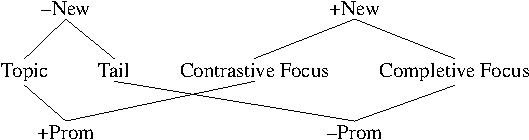
\includegraphics{pdf/choi.pdf}}}} 



Though the underlying framework is different, these LFG-based studies
also have implications for the current model.  First of all,
\citet{bresnan:mchombo:87} provides an analysis of information
structure in multiclausal utterances. They delve into how \isi{topic}
relations in \ili{English} and Chiche{\^w}a can be captured in several
types of multiclausal constructions such as embedded clauses, relative
clauses, and cleft clauses.\is{clefting} This highlights the
importance of capturing an information structure relation between a
subordinate clause and the main clause that the subordinate clause
belongs to. In other words, subordinate clauses constitute their own
information structure, but the relation to their main clauses
additionally needs to be represented with respect to information
structure.  This is discussed in more detail in Section \ref{9:ssec:binary}
and Section \ref{10:ssec:relative:background}.  Second, LFG-based studies deal
with a variety of constructions in the study of information structure,
whereas a large number of studies based on other frameworks treat only
simple declarative sentences. The construction types that LFG-based
studies address include interrogatives
(\textit{wh}-questions\is{\textit{wh}-questions} and
\textit{yes}/\textit{no}-questions), negation,\is{negation} clefts
\citep{king:95}, \isi{scrambling} \citep{choi:99}, and so-called
topicalization (i.e.\ \isi{focus}/topic \isi{fronting} in the present study)
\citep{man:07}.  Third, it is also noteworthy that LFG-based studies
tend to apply their formalism directly within a specific
language. Studies within other frameworks normally apply their
formalisms to \ili{English} first, and then project them analogously
into other languages. As a consequence, the analyses tend to be rather
dependent on English-like criteria. LFG-based work, on the other hand,
straightforwardly looks into how a language configures information
structure. LFG-based work on information structure has sometimes been
criticized for not treating prosodic factors significantly, but to my
understanding this is mainly because they do not start their work from
English, and as we have seen,\is{prosody} prosody is not heavily
responsible for information structure markings in a number of
languages (e.g.\ \ili{Chiche{\^w}a}, \ili{Korean}, and
\ili{Cantonese}).  Fourth, LFG-based studies take significant notice
of the mismatches between meanings and markings of information
structure and seek to reflect these discrepancies in their
formalism. Lastly, the present model is similar to
\citet{bresnan:mchombo:87} in that information structure is handled
within SYNSEM and an independent structure is therefore not needed.



\section{Summary}
\label{8:ssec:summary}

Since the pioneering work of \citet{engdahl:vallduvi:96}, information
structure has received attention in HPSG-based research.  The main
endeavor of these studies is to point out the necessity of viewing
sentential form in relation to information structure. This motivation
is also importantly applied to my model. Nevertheless, the present
study differs from previous studies in several key ways. First,
\isi{underspecification} is not widely used in the previous studies,
but the current model emphasizes underspecification as a key to the
representation of information structure. Second, while most previous
studies do not differentiate information structure marking and
information structure meaning, the two are entirely distinct in the
current model. Third, information structure is represented only under
CONT(ent) (i.e.\ MRS)\is{MRS} in the current model rather than in a
separate structure. Fourth, prosodic information is selectively
incorporated into the formalism, in accordance with what
\citet{bildhauer:07} suggests from a big picture perspective, but with
the direct application of his specific rules.  The implementation
details are discusses in the following chapters in addition to several
interesting points proposed in other frameworks. In particular,
inspired by the LFG-based studies, Chapter~\ref{chapter10-2} delves
into information structure with special reference to various types of
utterances (i.e.\ multiclausal constructions).

